\subsection{Excercise HelloWorld}
\label{sec:basic_hello_world_program}

\subsubsection*{Run Hello World}
After following the instruction in Mic-Con, the code is executed by running \texttt{go run main.go} in the terminal.
The code was executed twice: The first time the given code was executed leading to the output shown in figure \ref{fig:screendump_helloWorld_basicExecution}.
The second time the code was executed with different text, which can be seen in figure \ref{fig:screendump_helloWorld_differentText}.

\begin{figure} [h]
    \centering
    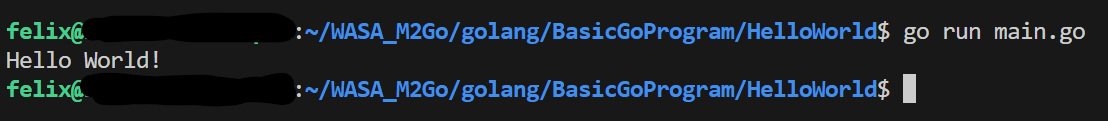
\includegraphics[width=0.8\textwidth]{figures/goLang/helloWorld/golang_helloWorld_basicExecution.png}
    \caption{Screendump showing the basic execution of the Hello World program}
    \label{fig:screendump_helloWorld_basicExecution}
\end{figure}

\begin{figure}[h]
    \centering
    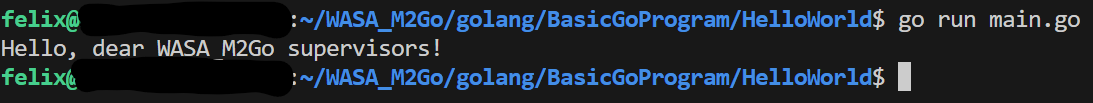
\includegraphics[width=0.8\textwidth]{figures/goLang/helloWorld/golang_helloWorld_ExecutionDifferentText.png}
    \caption{Screendump showing the execution of the Hello World program with different text}
    \label{fig:screendump_helloWorld_differentText}
\end{figure}

\subsubsection*{Code Explanation}
\begin{lstlisting}[
    language=Golang,
    caption={Hello World Program in Golang with explanations},
    label={lst:helloWorld},
    numbers=left,
    numberstyle=\tiny
    ]
    // main.go 
    // Author: Felix Weik

    package main    // package declaration: every executable belongs to the main package
                    // by declaring this package, a executable file is produced after compliation
    
    import "fmt"    // import the fmt package, a standard library package 
                    // implementing formatted I/O functions
                    // after import, one can use the functions of the imported package

    func main() {   // declares the function main, which is the 
                    // entry point of the program
        fmt.Println("Hello, World!")    // call the Println function 
                                        // of the fmt package; Println prints 
                                        // the given text to the standard output
    }               // end of the main function
    
\end{lstlisting}

\subsubsection*{HelloName}
The goal of this task is to extend the already given HelloWorld program to the HelloName program, prompting the user for a name then showing the given prompt in the output.
The code is shown in listing \ref{lst:helloName}:
\begin{lstlisting}[
    language=Golang,
    caption={Extension of helloWorld to helloName},
    label={lst:helloName},
    numbers=left,
    numberstyle=\tiny
    ]
    // main.go
    // Author: Felix Weik

    package main

    import (
        "fmt"
    )

    func main() {
        greet()
    }

    func greet() {
        var name string
        fmt.Print("What is your name? ")
        fmt.Scanln(&name)
        fmt.Println("Hello, " + name + "!")
    } 
\end{lstlisting}

The result of the executed code is shown in figure \ref{fig:screendump_helloName}

\begin{figure}
    \centering
    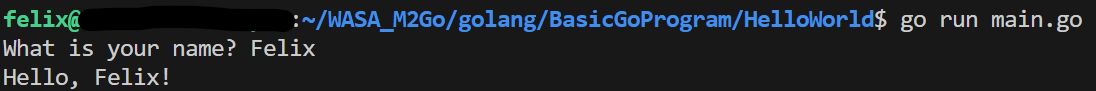
\includegraphics[width=0.8\textwidth]{figures/goLang/helloWorld/golang_helloWorld_helloName.png}
    \caption{Screendump showing the execution of the HelloName program}
    \label{fig:screendump_helloName}
\end{figure}